% Suppress some compilation warnings
\RequirePackage[save,showerrors]{silence}
\WarningFilter{biblatex}
  {The starred command '\DeclareDelimAlias*' is} % APA package is using this deprecated starred version
\WarningFilter{transparent}
  {Loading aborted} % Used by the svg package

\documentclass[usenames,dvipsnames,10pt]{beamer}

% languages typesetting rules
\usepackage[main=french,english]{babel}

% links configuration
\usepackage{hyperref} % commands such as \href, \url, etc.
\hypersetup{
    colorlinks=true,
    linkcolor=,
    urlcolor=NavyBlue,
    citecolor=Green
}

% bibliography configuration
\usepackage[style=lncs,backend=biber,backref=true]{biblatex}

\usepackage{csquotes} % biblatex extensions for non-english languages
\usepackage{caption} % more control over captions
\usepackage{subcaption} % for subfigures
\usepackage{ccicons} % icons for Creative-Commons licenses
\usepackage{hologo} % tex and co. logos
\usepackage{siunitx} % for displaying large numbers
\usepackage[inkscapepath=./build/svg-inkscape/]{svg}

\graphicspath{{images/} {../images}}

% Beamer theme configuration
\usetheme{metropolis}
\metroset{sectionpage=progressbar, progressbar=frametitle}
\setbeamertemplate{caption}[numbered] % Show figure number when using `\caption` instead of `\caption*`
\setbeamertemplate{footline}[page number] % Show the current page number in the bottom line of each slide
% \setbeameroption{show only notes}

% Bibliography configuration
\bibliography{../references.bib}

% Meta information about this presentation
\title{L'identification des projets de logiciel libre accessibles aux nouveaux contributeurs}
\titlegraphic{
\includegraphics[width=0.25\textwidth]{EIAH_2023}}
\institute[]{\href{https://creativecommons.org/licenses/by-sa/4.0/}{\ccbysa}}
\author{%
    Paul Hervot\inst{1}%
    \and%
    Benoît Crespin\inst{2}%
}
\institute{
    \textsuperscript{1} Laboratoire de Recherche de L’EPITA (LRE), 14-16 rue Voltaire, \\94270 Le Kremlin-Bicêtre, France
    \and
    \textsuperscript{2} Université de Limoges, XLIM/ASALI, UMR CNRS 7252, France
}
\date{15 juin 2023}

\newcommand{\mycite}[1]{%
    \citeauthor{#1} \citeyear{#1} \cite{#1}%
}

\begin{document}

\frame{\titlepage{}}

\section{Contexte}

\begin{frame}{Mémoire de Master}
    Formation d'ingénieur, enseignant à EPITA.

    Mémoire supervisé par Benoît Crespin.
    
    \note[item]{Très rapide, juste histoire de dire que je ne suis pas issu
    moi-même du milieu EIAH}
\end{frame}

\begin{frame}[fragile]{Contributions au logiciel libre}
    Nombreuses barrières d'accès, souvent discriminantes :
    \mycite{barriers-2018}, \mycite{newcomers-accessibility-2016},
    \mycite{newcomers-onboarding-2018}.

    \bigskip\bigskip

    Souvent liées aux propriétés des projets $\implies$ peut-on identifier
    lesquels sont accessibles ?

    \note[item]{%
        Même des projets populaires comme Apache Hadoop ont un très
        faible taux de rétention des nouveaux contributeurs, $82\%$ d'après
        Mendez et al. Les barrières sont très variées et sont souvent
        actionables par le projet lui-même : elles concernent la documentation
        disponible, la complexité des outils nécessaires et du setup à mettre en
        place pour commencer à travailler, ainsi que le comportement des
        mainteneurs.
    }
\end{frame}

\begin{frame}[fragile]{Inspiration}
    \mycite{signals-2019} : quels signaux utilisent les aspirants contributeurs.

    \begin{minipage}{.49\textwidth}
        \begin{figure}
            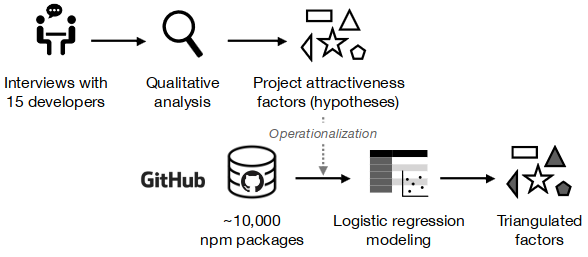
\includegraphics[width=\textwidth]{qiu_overview}
        \end{figure}
    \end{minipage}
    \begin{minipage}{.49\textwidth}
        \begin{figure}
            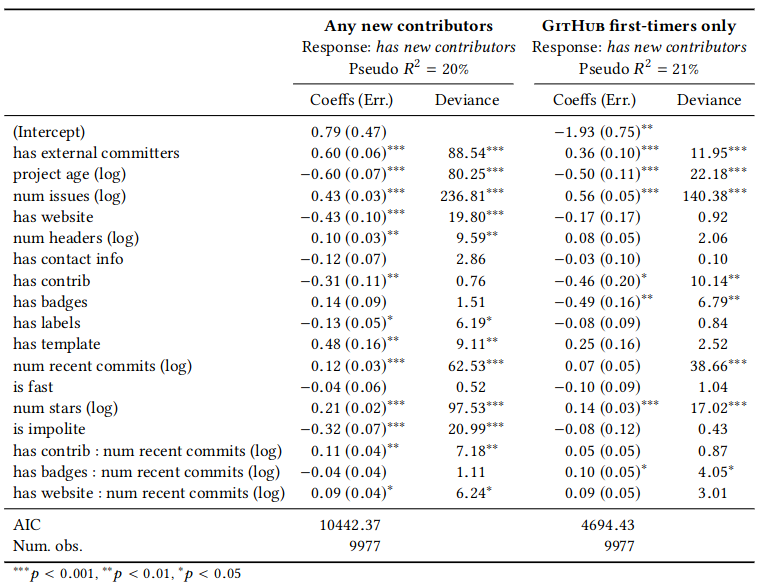
\includegraphics[width=\textwidth]{qiu_regressions}
        \end{figure}
    \end{minipage}

    \note[item]{%
        Je me suis beaucoup inspiré de cet article de Huilian Sophie Qiu et al.
        qui identifie certains signaux que les aspirants contributeurs regardent
        dans un projet pour choisir auquel contribuer, puis mesure la
        correlation qu'il y a entre ces signaux et la présence de tentative de
        contributions.

        Ils trouvent en particulier qu'un grand nombre de commits récents est
        lié à une meilleur attractivité, contrairement à la présence
        d'instructions de contribution. Leur étude mesure aussi de façon très
        intéressante l'impact de la politesse des mainteneurs, ce que mon
        approche ne me permettra pas de faire.

        Mon but est de vérifier si ces signaux marchent aussi pour identifier
        les projets \emph{accessibles} (les contributeurs arrivent à contribuer,
        leur code est merged dans le projet) et non seulement attractifs (les
        gens \emph{essayent} de contribuer).
    }
\end{frame}

\section{Méthodologie}

\begin{frame}[fragile]{Pour dépasser les limites de GitHub}
    \mycite{mining-github-2014}, \mycite{penumbra-oss-2022} : limites du minage
    mono-plateforme.

    \mycite{barriers-2018} : limites des études se concentrant sur quelques gros
    projets uniquement.

    \bigskip

    $\implies$ Besoin d'une stratégie de minage de données plus représentative
    et générique.

    \begin{figure}
        \includesvg[width=0.5\textwidth]{softwareheritage}
    \end{figure}

    \note[item]{%
        Autre objectif : dépasser les limites de l'analyse de données issues de
        GitHub (beaucoup de projets "personnels", beaucoup de PR non marquées
        comme merged alors qu'elles l'ont été à la main, etc.).
    }
\end{frame}

\begin{frame}{Pertinence pour la recherche}
    \mycite{swh-2019}, \mycite{swh-seirl}.

    \begin{itemize}
        \item $+$\num{239000000} projets
        \item $+$\num{3000000000} \emph{commits} uniques
        \item Parcours régulièrement Bitbucket, GitHub, gitlab.com, CRAN, Maven,
            gnu.org, NPM, pypi, sourceforge, \ldots
        \item google code, autres GitLabs, autres origines à la demande
    \end{itemize}

    \note[item]{%
        Software Heritage maintien la plus grande archive logicielle publique au
        monde avec l'objectif spécifique de la rendre exploitable à des fins de
        recherche. L'archive contient des projets issus de nombreuses sources
        différentes (GitHub restant la principale), y compris venant de
        logiciels de versionnement différents, et tous représentés sous un seul
        grand graphe de commits dédupliqués.
    }
\end{frame}

% TODO : présenter le graphe et la façon dont je le parcours

\section{Résultats}

\begin{frame}{Traitement de la présence d'instructions de contribution}
    \begin{figure}
        \begin{subfigure}[t]{0.45\textwidth}
            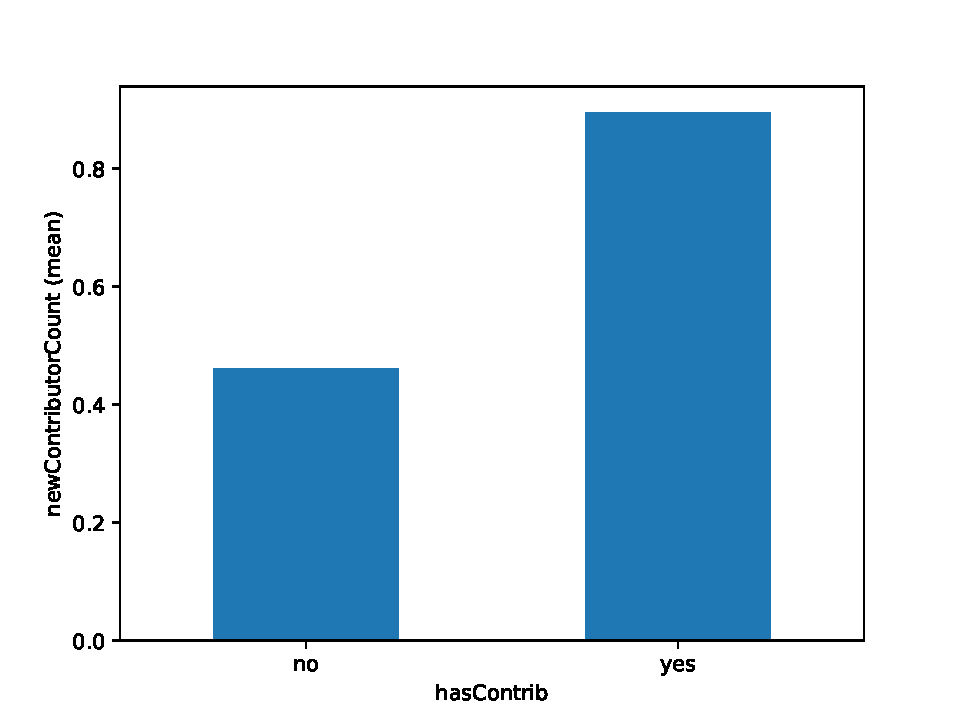
\includegraphics[width=\textwidth]{../experiment/data_analysis/hasContrib_meanNewContributorCount}
            \caption{Moyenne du nombre de nouveaux contributeurs pour chaque catégorie}
        \end{subfigure}
        \begin{subfigure}[t]{0.45\textwidth}
            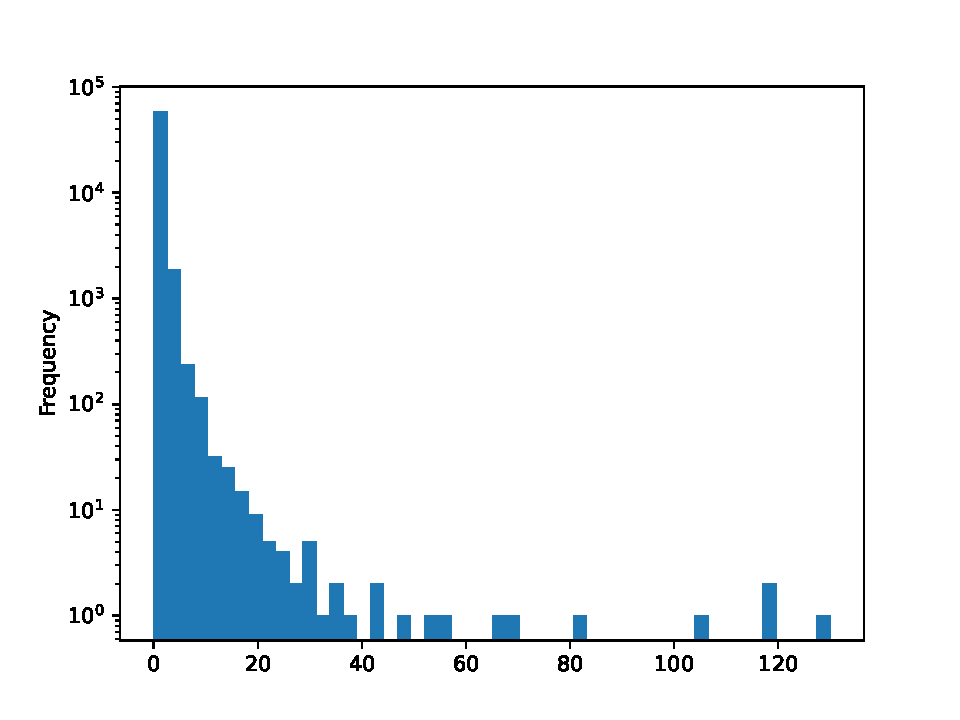
\includegraphics[width=\textwidth]{../experiment/data_analysis/newContributorCount_distribution}
            \caption{Nombre de nouveaux contributeurs\\(ordonnées logarithmiques)}
        \end{subfigure}
    \end{figure}
\end{frame}

% TODO : montrer les deux autres résultats

\begin{frame}{Contact}
    \begin{itemize}
        \item Contact : \href{mailto:paul.hervot@epita.fr}{paul.hervot@epita.fr}
        \item Dépôt GitHub :
            \href{https://github.com/Dettorer/synva-dissertation}{Dettorer/synva-dissertation}
        \item \emph{Replication package} :
            \href{https://zenodo.org/record/7023495}{zenodo.org/record/7023495}
    \end{itemize}

    \note[item]{%
        J'ai essayé de rendre le code le plus lisible et réutilisable possible.
    }
\end{frame}

\section{Bibliographie}

\begin{frame}[allowframebreaks]{Bibliographie}
    \printbibliography{}
\end{frame}

\end{document}
